%%%%%%%%%%%%%%%%%%%%%%%%%%%%%%%%%%%%%%%%%%
% INITALIZATION AND PACKAGES
%%%%%%%%%%%%%%%%%%%%%%%%%%%%%%%%%%%%%%%%%%

\documentclass[11pt]{article} % Define the class of the document

\usepackage{geometry}                
\geometry{a4paper} % Set A4 format for the paper                   

\usepackage{graphicx} % Include pictures

\usepackage{amssymb} % Math functions
\usepackage{amsmath} % Math functions

\usepackage{epstopdf}

\usepackage{enumerate} % Different enumeration types

\usepackage{color} % Allowed for colored text

\usepackage[numbered, autolinebreaks, useliterate]{mcode} % for including MATLAB code

\usepackage[final]{pdfpages} % Include full PDF pages to be incorporated

\usepackage[nottoc,numbib]{tocbibind} % Include the references in the table of content

\usepackage[labelfont=bf, justification=]{caption} % Put 'figure' of caption in bold and justify as centered

\DeclareGraphicsRule{.tif}{png}{.png}{`convert #1 `dirname #1`/`basename #1 .tif`.png}

\setlength{\parindent}{1cm} % Set an indentation for every paragraph in the document


%%%%%%%%%%%%%%%%%%%%%%%%%%%%%%%%%%%%%%%%
% START THE DOCUMENT
%%%%%%%%%%%%%%%%%%%%%%%%%%%%%%%%%%%%%%%%

\begin{document}


\thispagestyle{empty}

\begin{center}

\includegraphics[width=5cm]{ETHlogo.eps}

\bigskip
\bigskip
\bigskip


\LARGE{ 	Lecture with Computer Exercises:\\ }
\LARGE{ Modelling and Simulating Social Systems with MATLAB\\}

\bigskip
\bigskip
\bigskip
\bigskip

\small{Project Report}\\

\bigskip
\bigskip
\bigskip


%\begin{tabular}{|c|}
%\hline
%\\
%\textbf{\LARGE{Inter-State Collaboration Following a}}\\
%\textbf{\LARGE{Zombie Outbreak}}\\
\huge{\bf{Zombie Outbreak:\\The Effect of Inter-State Collaboration on the Survival of Humanity}}
%\\
%\hline
%\end{tabular}

\bigskip
\bigskip
\bigskip


\small{by\\}
\bigskip
\bigskip
\LARGE{Matthieu G. \textsc{Mottet}\\Basile I. M. \textsc{Wicky}}

\bigskip
\bigskip
\bigskip
\bigskip
\bigskip
\bigskip
\bigskip
\bigskip
\bigskip
\bigskip
\bigskip
\bigskip
\bigskip
\bigskip
\bigskip
\bigskip
\bigskip
\bigskip
Zurich\\
December 2012\\

\end{center}


 % Load the cover generated separately
\newpage

\section*{Agreement for free-download} % * removes it from the table of content
\thispagestyle{empty} % Remove page number here

\bigskip
\bigskip

\large We hereby agree to make our source code for this project freely available for download from the web pages of the SOMS chair. Furthermore, we assure that all source code is written by ourselves and is not violating any copyright restrictions.

\begin{center}

\bigskip
\bigskip

\begin{tabular}{@{}p{2cm}@{}p{6cm}@{}@{}p{6cm}@{}}
\begin{minipage}{3.3cm}
\end{minipage}
&
\begin{minipage}{6cm}
\vspace{3cm} \large{Matthieu G. \textsc{Mottet}}

\vspace{\baselineskip}

\end{minipage}
&
\begin{minipage}{6cm}

\vspace{3cm}\large{Basile I. M. \textsc{Wicky}}
\vspace{\baselineskip}
\end{minipage}
\end{tabular}


\end{center}
\newpage

% ETH DECLARATION OF ORIGINALITY
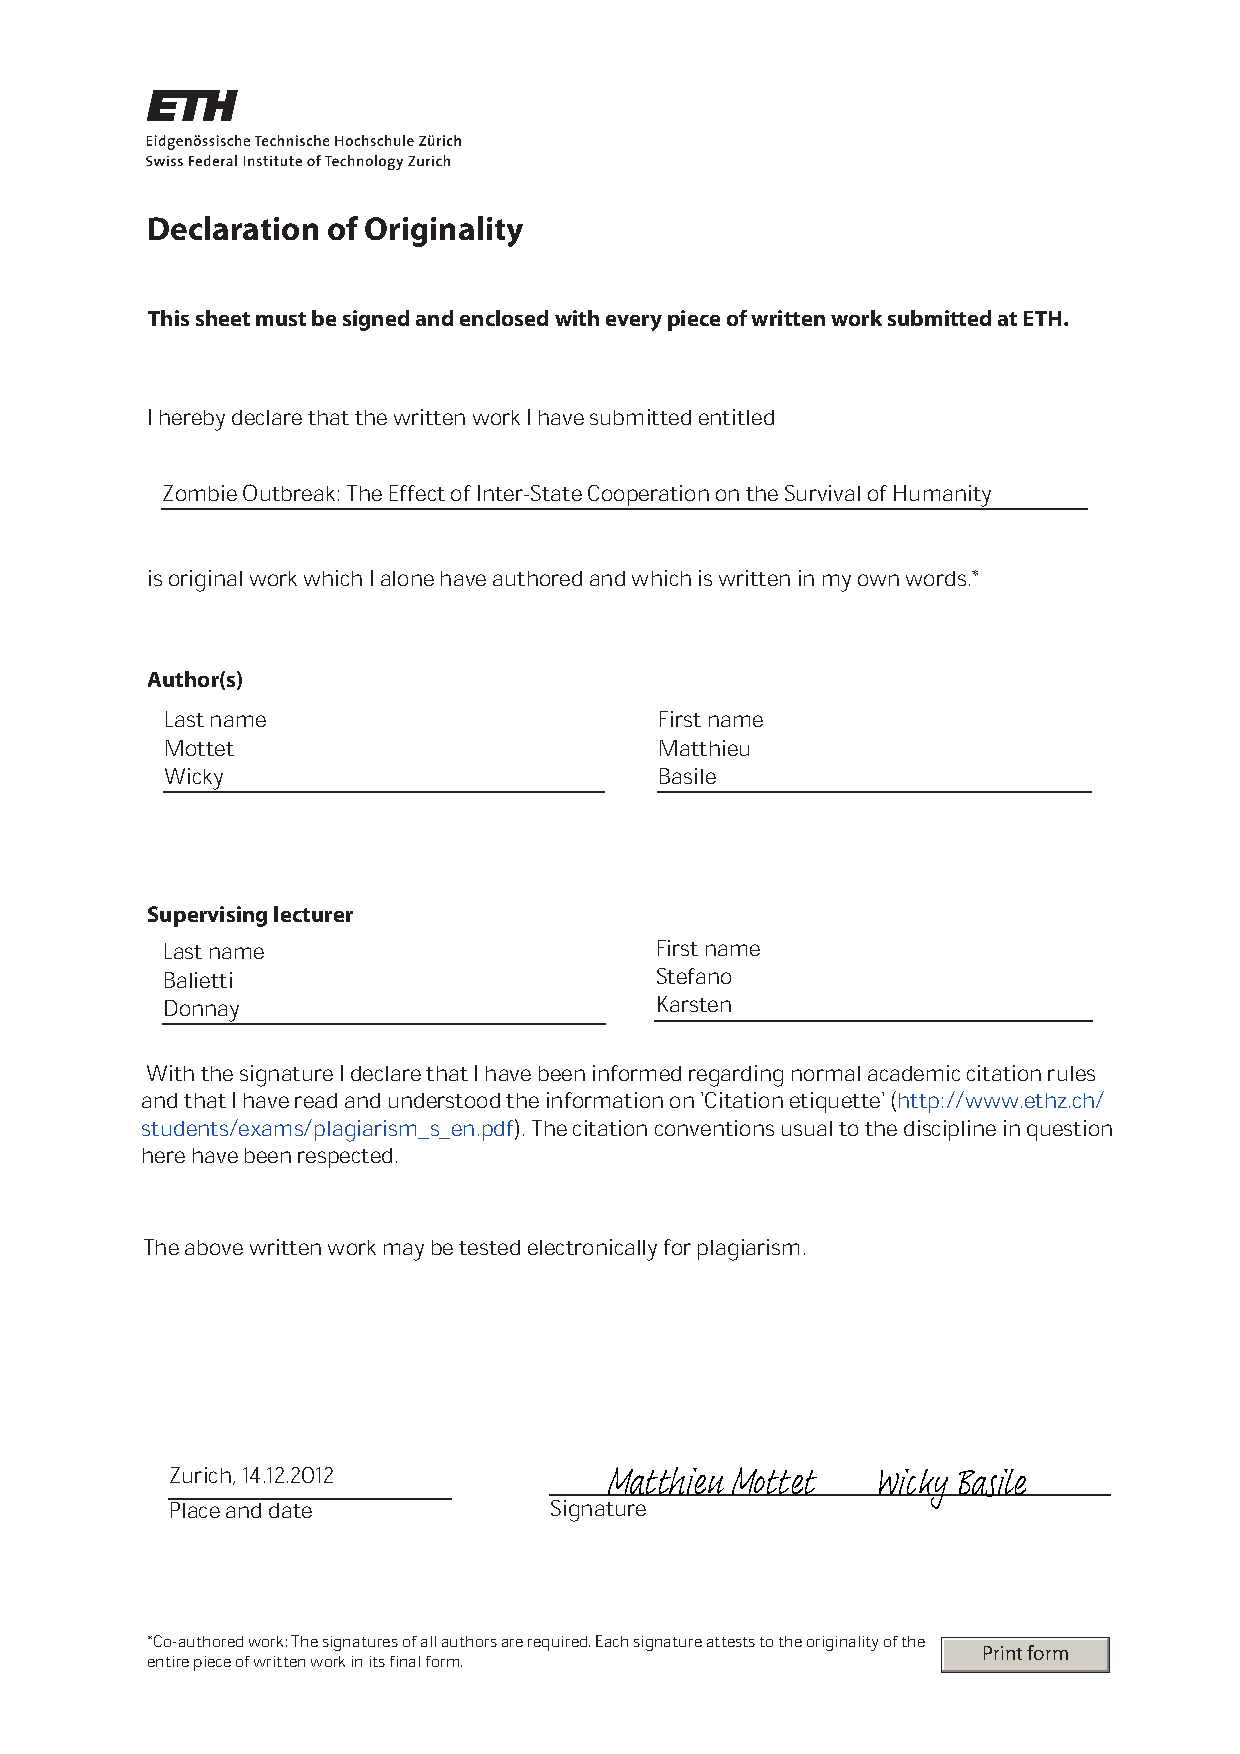
\includepdf{confirmation_en.pdf}

% TABLE OF CONTENT
\tableofcontents




% ABSTRACT 
\newpage

\section{Abstract}\indent
\textcolor{red} {This part needs updating once the rest of the report will be finished}\\
Investigation of the application of the SIR model to a zombie outbreak has already been studied, raising the fear of dark days for humanity. However, we would like to deepen this investigation to a multi-state system to see how interactions between subpopulation may brighten the future of the human race. Moreover, we are interested in seeing to what extent the different paradigms of international politics, Realpolitik, Liberalism and Neoconservatism as defined by Daniel W. Drezner in Theories of International Politics and zombies may lead to different outcomes.

% INDIVIDUAL CONTRIBUTION
\section{Individual contributions}\indent

M.G.M. and B.I.M.W. formulated the question in mathematical terms and discussed the implementation in MATLAB. M.G.M. wrote the code. M.G.M. and B.I.M.W. analysed and discussed the results and B.I.M.W. wrote the report.

% ACKNOWLEDGMENTS
\section{Acknowledgments}\indent

We wish to thank Karsten Donnay and Stefano Balietti for their support in our work, fruitful discussions and open-mindedness to accept such a project. We also would like to thank the Chair of Sociology for the computational support provided with simulation time on the ETH cluster Brutus.



% INTRODUCTION AND MOTIVATION
\newpage
\section{Introduction and Motivations}\indent

\subsection{Zombie Outbreak}\indent

While models of international relationship have already been studied under different pressure components, the effect of a zombie outbreak on international collaboration and equilibrium is a question that has been underestimated and was never addressed to the best of our knowledge. It is remarkable that the effect of such an intense event has not been looked at, although the fear of zombies and the threat they represent is vivid for many of us as reflected by the importance of the zombie culture. Zombies, compared to other unnatural creatures such as vampires or aliens, have the very peculiar property not to be a minority inside the human civilization but rather to be in a way a part of it, just not quite as it was, i.e. zombified. Accordingly, zombies cause a much more deep-rooted fear as they not only threaten our lives but also the our very sense of identity as it questions our notion of what humanity is. The psychological effect of such a non-standard threat as well as the repercussion on the behaviour of large popluation systems such as states should be far from trivial. Accordingly, we decided to simulate an inter-state collaboration models in order to see the outcome on a large scale of such an extreme event. While some people might question the validity of such a study (no zombie has been observed so far), we think that the applicablity of such a reasoning could extend to a more probable large-scale epidemological disaster or simply, give a line of reasoning to cope with what former U.S. Secretery of Defense Donald Rumsfeld referred as the "unknown unknowns" of international security. Zombies might not be real, but the threat and stress they could impose on current world politics is. \\

\subsection{Epidemological Studies}\indent

Epidemiological models have been well studies to see the evolution dynamics and spread of a disease in a population \textcolor{red}{REFERENCE}. They are based on a mass action model where interaction between susceptibles and infected together with an infection constant define the rate of infection. In the simplest case of such models, infected people can move to the immunized category also following a mass action law. This models have been shown to work in numerous cases and  when corrections are added \textcolor{red}{REFERENCE}, they can very well represent the evolution and spread of an infectious disease in a population. However, an epidemiological model of communicating population has not been tested to the best of our knowledge. \\

\subsection{Zombies: a Definition}\indent

The origin of the word "zombie" as well as its initial meaning is quite remote from modern pop culture description. The word itself is said to have originated in the voodoo language in the Caribbean \cite{drezner}. The original description is that of a ritual where the wizard of a tribe would start controlling another person. The fact that this person doesn't have a soul anymore and that it is no under the control of another human being, i.e. it has no longer a free-will, makes it a zombie \cite{drezner}. Some studies suggest that those "zombified" members of the tribe where actually administrated a cocktail of two natural drugs, one being a neurotoxin and the other a hallucinogenic drug \textcolor{red}{REFERENCE}. In fact, the neurotoxin damages the brain and turns the person into a vegetative state.\\



Zombies in popular culture differ a lot from this original etymological definition. The canon of the zombie literature have had numerous description and hypothesis on how they may emerge in a human population, as well as what might characterize them. Since Romero's "night of the living dead" \textcolor{red}{REFERENCE}, where zombies were said to have raised from some pseudo-magical event, the depiction and origin of zombies has considerably evolved. Recent zombie stories usually describe the genesis of flesh-heating monsters in an epidemiological sense, typically some sort of virus. Recent examples in the zombie culture are numerous and include (non-exhaustively) "Resident Evil", "28 Days Later". For simplicity, we will treat the emergence and zombification events as linked to an infectious disease of some sort, allowing the treatment of the problem with a modified epidemiological model. The big difference with a standard infectious disease where people usually get immunized, being transformed into a zombie is a on way process. The only way out is death and therefore, humans (susceptibles) can only decrease in our system.\\


\subsection{Popular Believes in the Event of the Zombie Outbreak}\indent

It is interesting to notice that most zombie canon predict a very bleak outcome concerning the fate of humanity. Indeed, most movies/film describe an almost total disappearance of humans and the few survivors are rarely in a position that seem to be about to brighten up. While some might argue that the disappearance of humanity might not be such regretful event and might actually benefit our planet \textcolor{red}{REFERENCE}, we decided to see if the usual outcome and fate of the human race in case of a zombie outbreak might differ from those classical scenarios, and if so, under which set of particular conditions. 

Mathematical modeling of a zombie outbreak in a single population has previously been simulated \cite{munz2009zombies} but showed very little hope for humans in the case of such an unlikely event. The primarily reason for the annihilation of humans in all of the presented scenarios lies in their models. In contrast to "classical" epidemiological models where infected people can recover and although having changed population statues (going from susceptible to removed in a immunized sense of the term), they do not actually die. This is very different for the zombie scenario, where now "removed" is no longer synonym of "immunized", but is actually a very nice way of putting "dead". Accordingly, under the considerations of the model presented, humans can only day and this eventually happens in every case (some set of parameters can give reprieve the inevitable fate).\\

\subsection{Can a Different Treatment of the Problem Lead to a Different Outcome?}\indent

We rationalized that a more state-based description of the world population might actually help in brightening the outcome of a zombie outbreak. In fact, the world in divided into states and nations that apply their own laws and restrictions in terms of immigration. If immigration applies to humans, it might as well apply to zombies. In such a case, one might envision that in a given state under the threat of a zombie epidemiological disaster, flux of incoming susceptibles to help them kill the zombies or on the other hand the emigration of the survivors to a non-infected state might lead to various outcome. For example, it is imaginable to see the emergence of a zombie-only state where all the remaining survivor would have found shelter in another state. Or even better, that the help of susceptible from another state might help eradicate the new-coming zombie threat. 

For those reason we decided to simulate a model of interacting sub-populations, each under an epidemiological-like treatment. The inner-state epidemiological model describes the emergences of zombies from a spreading disease point of view, while the populations fluxes between states would represent immigration/emigration of the populations under concern (humans and/or zombies). 

Moreover, we are interested in seeing to what extent the different paradigms of international politics, Realpolitik, Liberalism and Neoconservatism as defined by Daniel W. Drezner in Theories of International Politics and zombies may lead to different outcomes.
Expected Results

As describe in Drezner's book, we except different equilibrium outcomes depending on the paradigm under consideration. He postulates the possibile appearance of zombie states under Realpolitik and Liberalism paradigms while Neoconservatism would not allow such an outcome.

% DESCRIPTION OF THE MODEL
\newpage
\section{Description of the Model}\indent

In order to simulate a multi-state system under epidemiological evolution we needed to define a clear mathematical framework treating both the population fluxes within states and among states. Such a treatment was necessary to represent the two-fold problem of a zombie outbreak at an international level:
\begin{enumerate}[i.]
	\item Intra-state fluxes have a fixed physical definition and are invariable among states. They represent the true epidemiological part of our model
	\item Inter-state fluxes do not have a similar physical meaning and will depend greatly on the paradigm of international politics under consideration (\textit{Realpolitik}, Liberal, Neoconservatorism). They do not represent epidemological variation \textit{per se} but modelisation of immigration/emigration fluxes.
\end{enumerate}

With such an approach, we would be able to separate the population evolutions at the international and domestic level. We decided to simulate the microstate level under a modification of the classical SIR model \textcolor{red}{REFERENCE} called the SZR model (S for susceptible, Z for Zombies, R for removed) \cite{munz2009zombies}. Contrary to the 

\subsection{Microstate Description}\indent

\subsection{Macrostate Description}\indent






\begin{figure}[h!]
%\centerline{
%includegraphics[scale=0.15]{Images/Zombie_model.png}}
\caption{Schematic of our model including all variables. The parts in blue represent the fluxes at the microstate level while the parts in orange represent the macrostate population fluxes. This schematic represent our simulated system where the interaction of three states (microstates) is modeled \label{overallmodel} }
\end{figure}

\begin{equation}  \label{eq:smicro}
\Delta S_{i}^{micro} = -\alpha S_{i} Z_{i} -\gamma S_{i} Z_{i} = -(\alpha + \gamma) S_{i} Z_{i}
\end{equation}

\begin{equation} \label{eq:zmicro}
\Delta Z_{i}^{micro} = +\alpha S_{i} Z_{i} - \beta S_{i} Z_{i} = (\alpha - \beta) S_{i} Z_{i}
\end{equation}

\begin{equation} \label{eq:rmicro}
\Delta R_{i}^{micro} = +\beta S_{i} Z_{i} + \gamma S_{i} Z_{i} = (\beta + \gamma) S_{i} Z_{i}
\end{equation}

\begin{equation} \label{eq:smacro}
\Delta S_{i}^{macro} =  \sum_{j\neq i}{ \left( \nu \langle \Delta S_{j} \rangle - \nu  \langle \Delta S_{i} \rangle \right) }
\end{equation}

\begin{equation} \label{eq:zmacro}
\Delta Z_{i}^{macro} = \sum_{j\neq i}{\left( \eta Z_{j}\tanh \left( \frac{Z_{j}}{S_{j}}\right) -\eta Z_{i}\tanh \left( \frac{Z_{i}}{S_{i}}\right) \right)}
\end{equation}



% IMPLEMENTATION
\newpage
\section{Implementation}\indent

the first equation is \eqref{eq:smicro}, the second is \eqref{eq:zmicro} and so on

The implementation in MatLab works on two levels: one taking care of the simulation of the epidemiological model, the other one taking care of the sweeping of the epidemiological parameters. We will discuss the key parts of the implementation as well as some of the interesting details that had to ensure the coherence of the model.


\subsection{The Outbreak Function}\indent

The outbreak function is the wrapping function of the epidemiological model. It first evaluates the different parameters, initialize the different matrices used throughout the simulation, calls the update function of our model and is finally responsible for the validation of the new data generated after each update cycle. The validation of the data allows to test if it worth continuing the simulation or if it should be shut down. This allows to save computational time. We implemented three exit policies in the simulation loop. First of all, we implemented two obvious safeguards when either the susceptible or the zombie population reaches zero. Continuing the simulation in either case would not make sense since the system already reached its final state. The third one is triggered when the different population evolution becomes too slow, indicating a relative steady state. Even though it might not be a true dynamical equilibrium, very little population variation over a very long time would not be of any significance within the framework of our model (e.g. a single zombie killing thousands of remaining humans over the course of a very long simulation simply because the infection to death rate as a particular value). In order to avoid unphysical convergences, we define the following control:

\begin{equation} \label{eq:outbreakequilibrium}
\left\langle \left| \Delta S \right| \right\rangle < x\ \&\&\ \left\langle\left|\Delta Z \right| \right\rangle < x
\end{equation}

Where $x$ is the threshold value. The mean of the absolute variation of susceptibles and zombies on the last 100 steps is calculated using a sliding window and compared to a threshold $x = 0.1$. If the values are smaller than the threshold, we assume a steady state or "quasi-equilibrium" and exit the simulation. Furthermore, a maximum number of step can be defined (default: $10^8$ steps) as last exit condition. Details of the code can be found in Appendix 10.1.

\subsection{The Update Function}\indent

The update function takes care of the evolution of the different populations at each cycle. It applies the different equations of the models and uses safeguards to avoid unphysical results. It first calculates the the variation-to-be of each population of each state based on the current populations. It does this in a sequential manner, first the susceptibles and then the zombies. After the update, it checks for the actual variations obtained. This is done in order to ensure that variations larger than the actual population size cannot occur.
The first constraint is applied during the computation of the flux exiting each states. Due to the structure of the program, negatives population values can arise. Though these populations will be extremely small ($> - 10^{-4}$), resulting in small negative exiting flux, they will lead to negative entering flux in the other states. These flux being considered as positive into the next control procedure, negative values have to be avoided.

The second constraint is applied after the computation of all flux. There is the possibility for the negative flux (death, contamination, emigration) to be bigger than the population plus the positive flux (immigration). In such case, we apply a simple algorithm to avoid the negative population:
\begin{enumerate}
	\item the negative flux are normalized and multiplied by the population plus the positive flux,
	\item the incoming flux of the two other states are corrected to fit the values,
	\item the validation is applied to the two other states.
\end{enumerate}
This algorithm is applied until all discrepancy is removed. Note that negative values up to $10^{-4}$ are allowed and that during the first step of the algorithm, in the case where the sum of the population and incoming flux is negative, this value is zeroed. This method allows a relatively fast convergence of the values while retaining physical significance of the model and its implementation. Details of the code can be found in Appendix 10.2.

\subsection{The Sweep Function}\indent

The sweep function acts as a wrapper function for the sweeping of each parameters between two values using defined steps. The results of each individual simulation is stored in a dedicated folder. It also assigns a id string to the sweep. This id allows to resume the sweep with the first non completed simulation, this feature was added due to the duration of the sweep with sufficient resolution. Details of the code can be found in Appendix 10.3.
% SIMULATION RESULTS AND DISCUSSION
\newpage
\section{Simulation Results and Discussion}\indent

\subsection{Population Time-Evolution under Different Regimes}\indent
 
% Doomsday figure
\begin{figure}[h!]
\centerline{
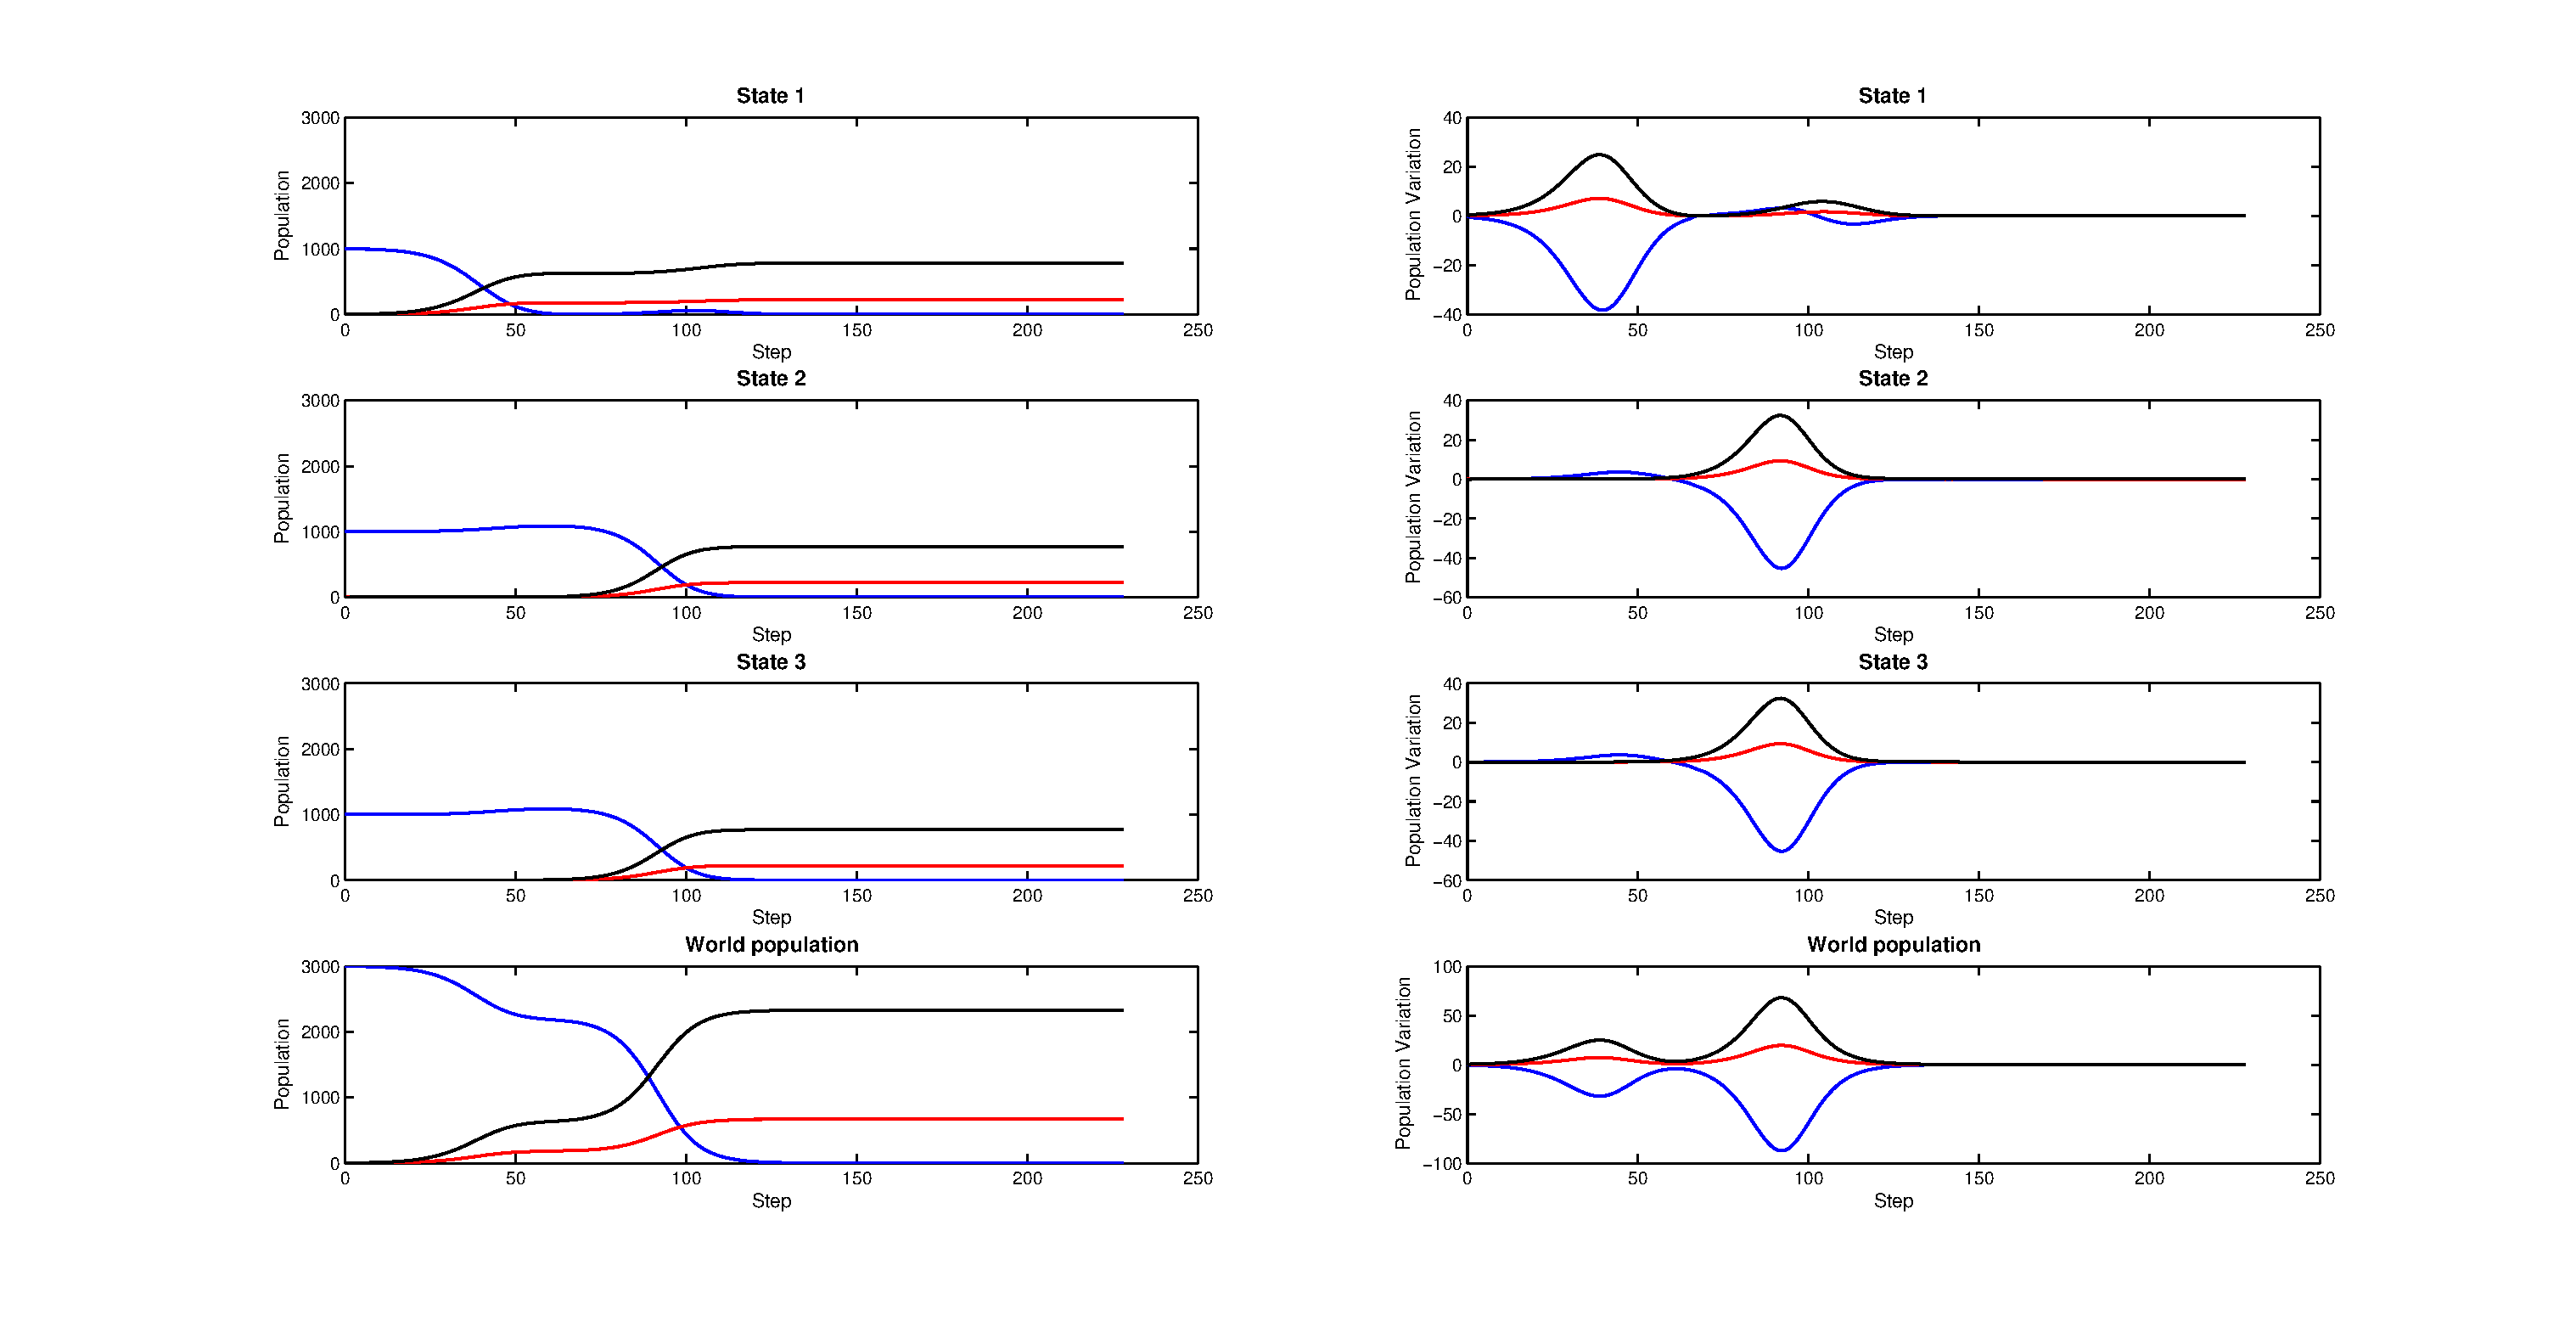
\includegraphics[scale=0.35]{Images/example_doomsday.eps}}
\caption{Doomsday scenario. Emergence of zombies in state 1 leads to full contamination of the world's population (\textcolor{blue}{blue} = susceptibles, \textcolor{red}{red} = zombies, black = removed, $\alpha=1.5\cdot10^{-4}, \beta=5\cdot10^{-6}, \gamma=5\cdot10^{-4}, \nu=0.1, \eta=1.5\cdot10^{-4}$). \label{doomsday} }
\end{figure}

% Zombie kill figure
\begin{figure}[h!]
\centerline{
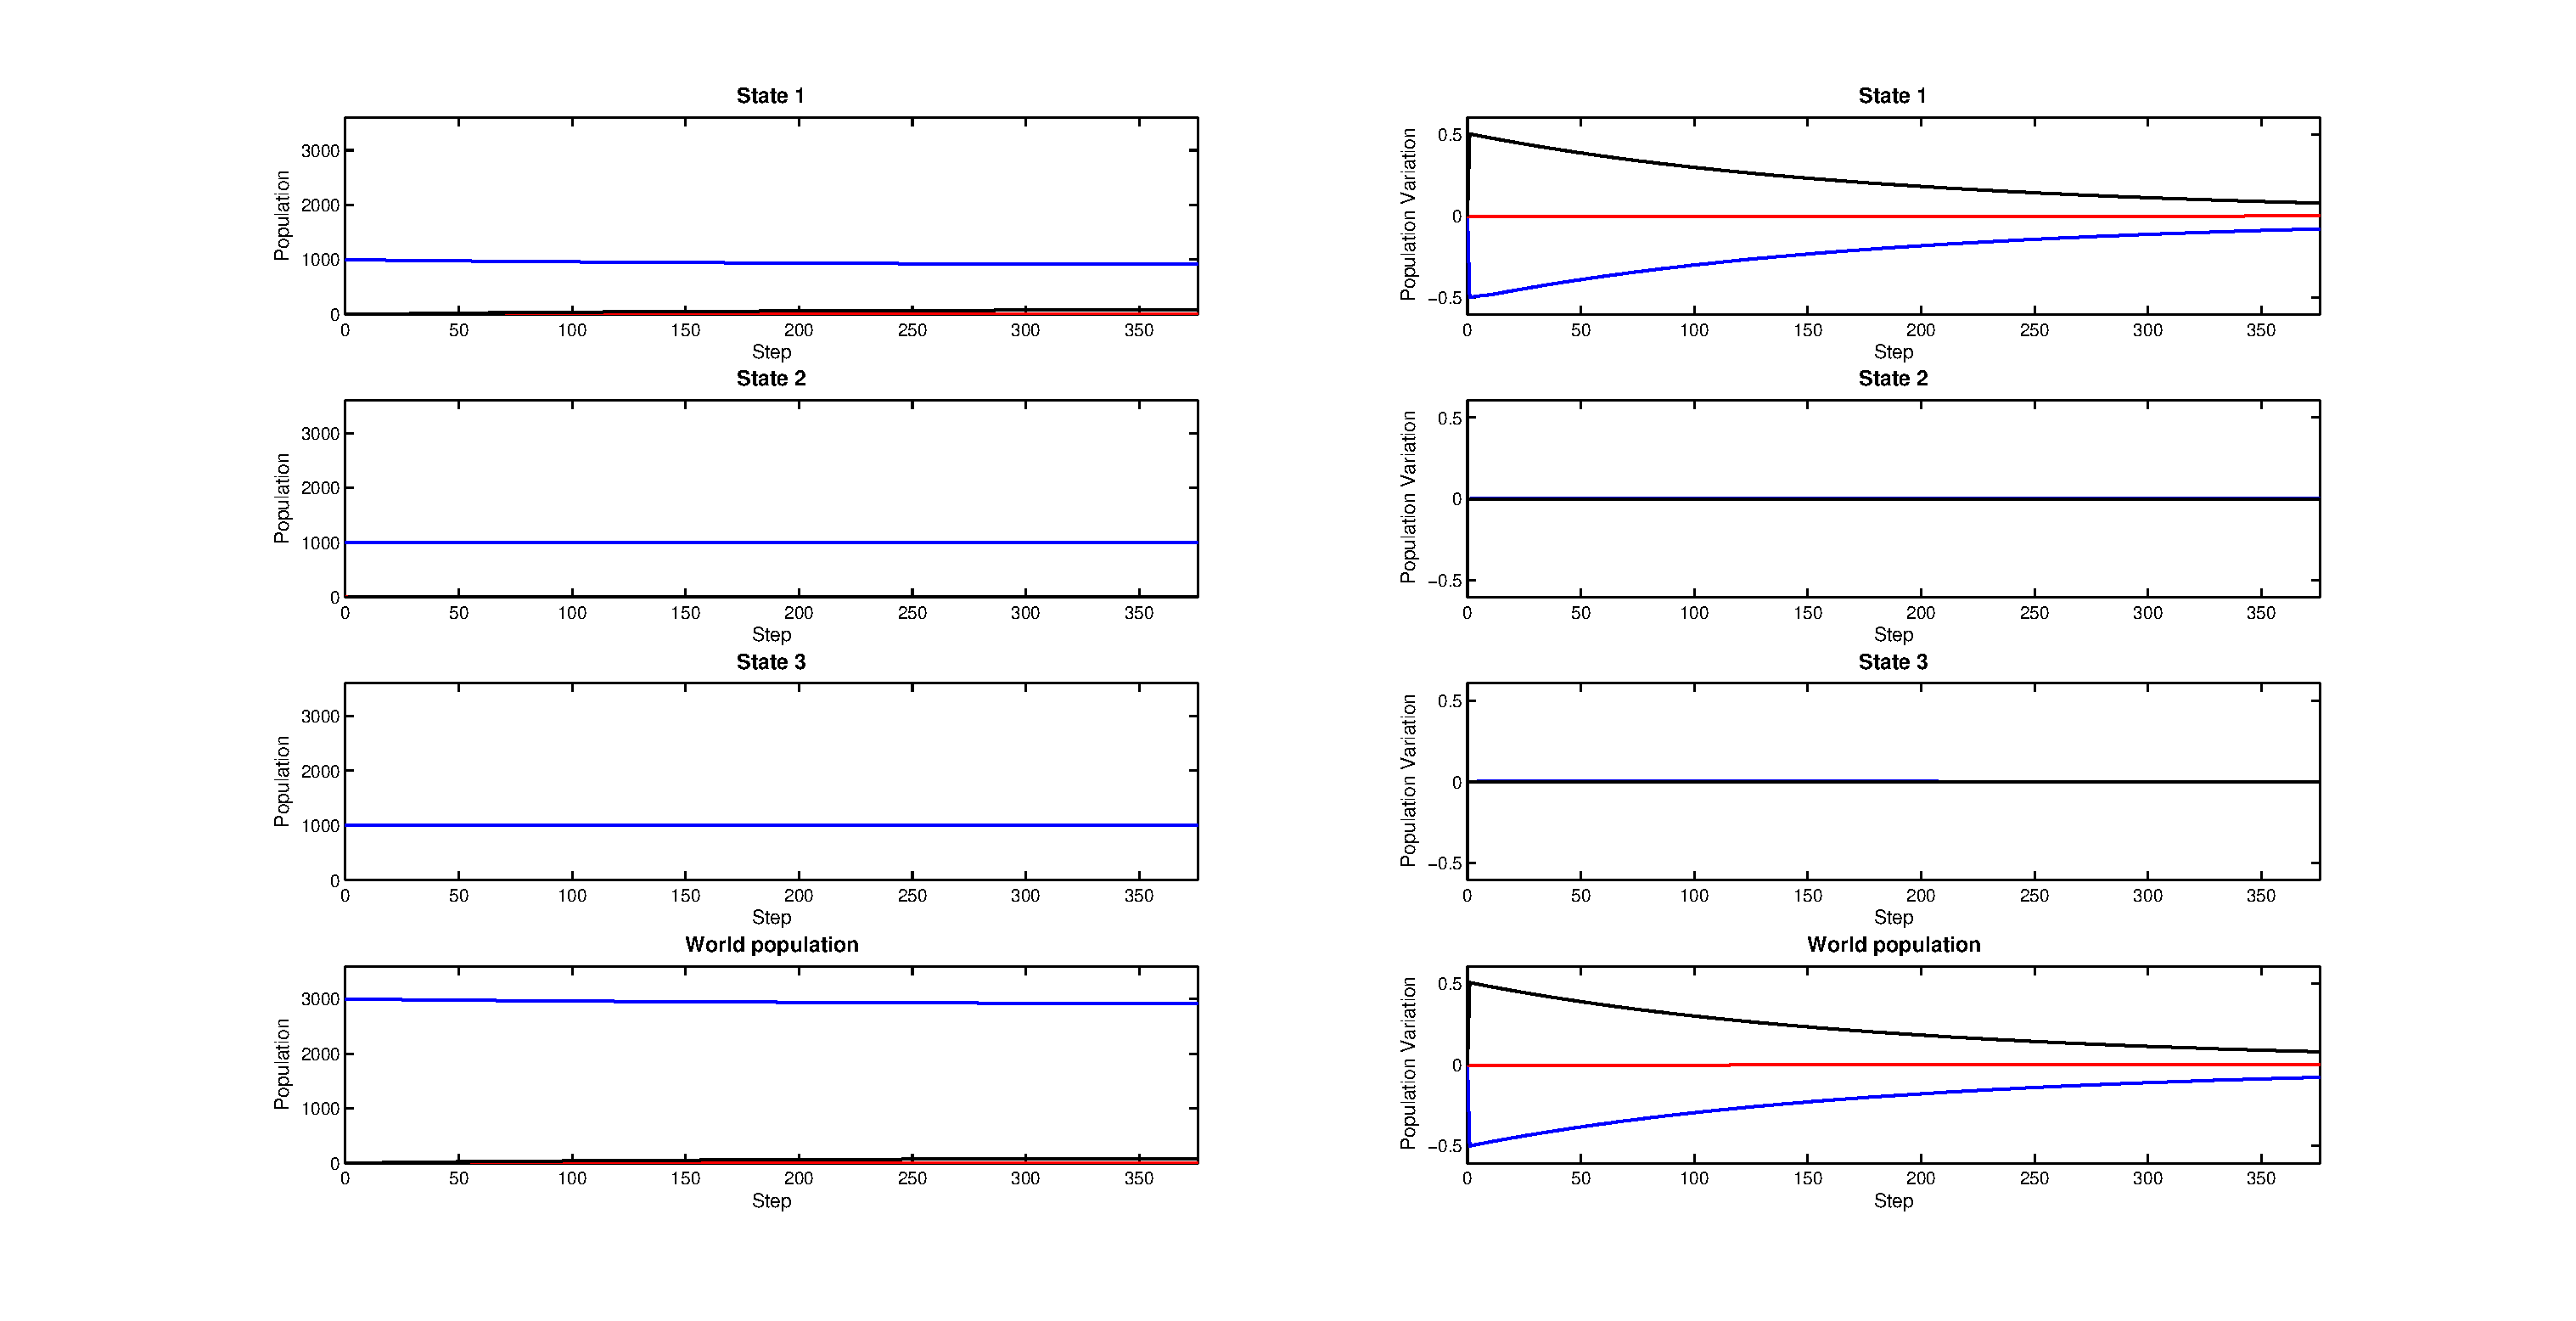
\includegraphics[scale=0.35]{Images/example_zkill.eps}}
\caption{Survival of humanity by zombie eradication. As soon as zombies appear in state 1, they get killed until the outbreak is contained  (\textcolor{blue}{blue} = susceptibles, \textcolor{red}{red} = zombies, black = removed, $\alpha=1.5\cdot10^{-8}, \beta=5\cdot10^{-6}, \gamma=5\cdot10^{-4}, \nu=0.01, \eta=1.5\cdot10^{-4}$).
\label{skill} }
\end{figure}

% Exode figure
\begin{figure}[h!]
\centerline{
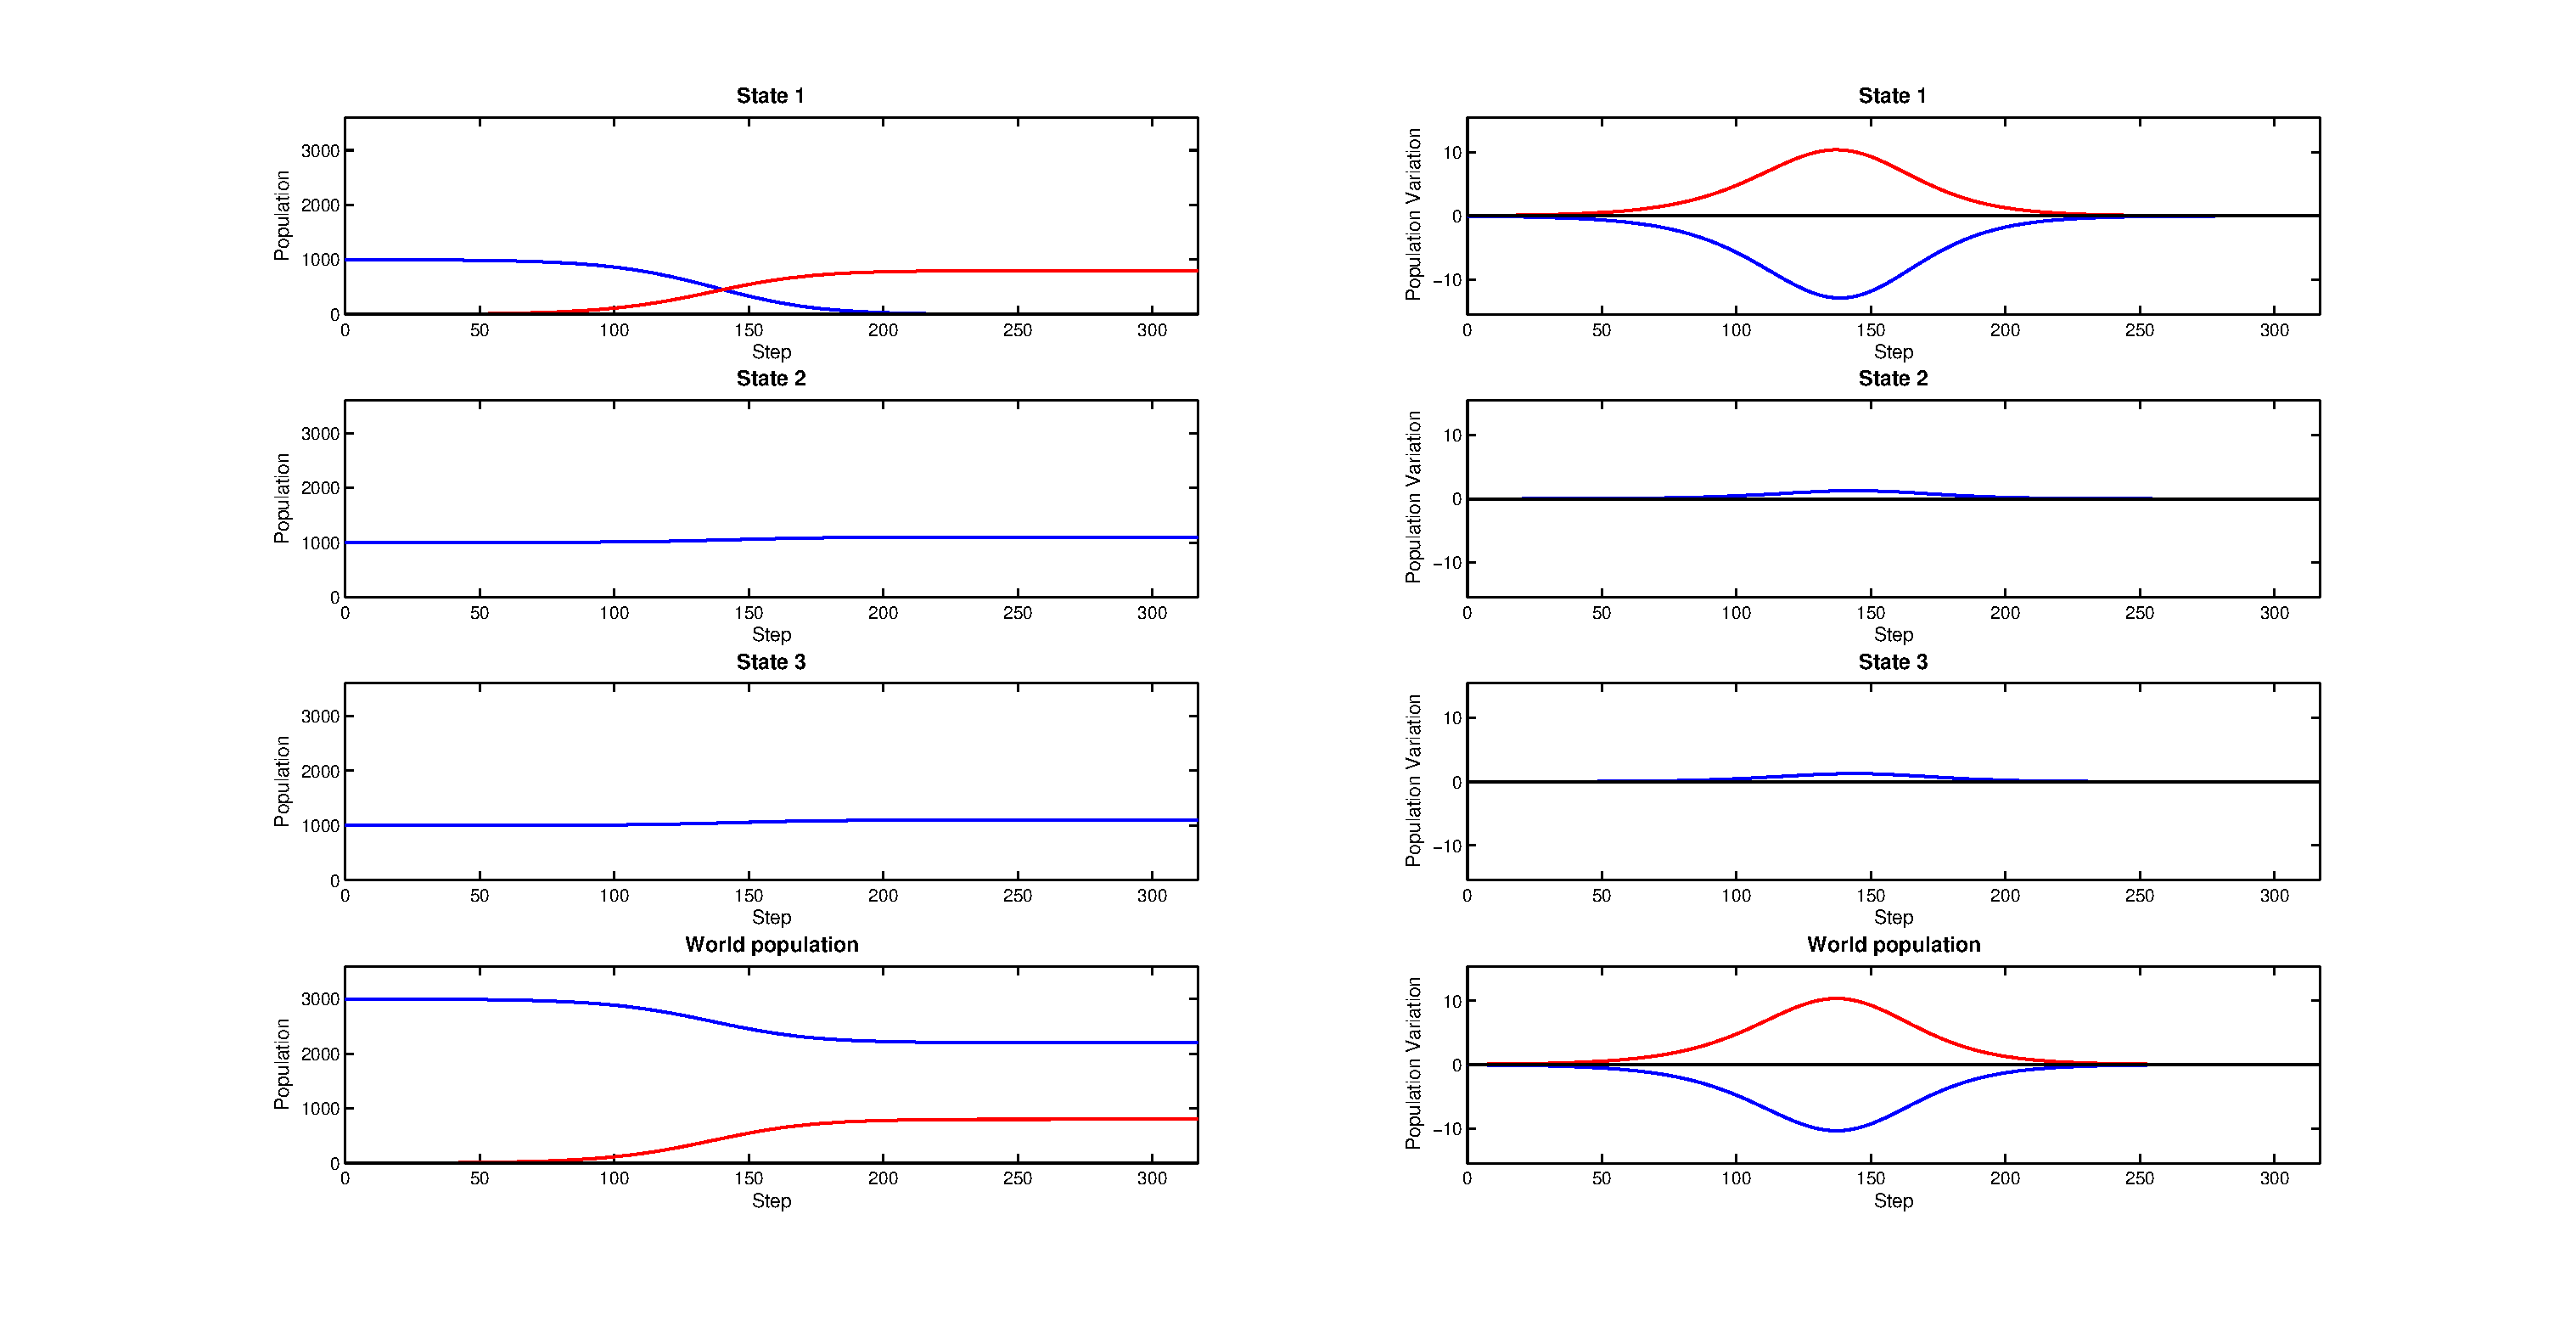
\includegraphics[scale=0.35]{Images/example_exode.eps}}
\caption{Survival of humanity and emergence of a zombie state. Emergence of zombies in state 1 leads to the exodus of the remaining population to states 2 and 3. State 1 then becomes fully infested of zombies and the remaining of the world's population is in state 2 and 3 (\textcolor{blue}{blue} = susceptibles, \textcolor{red}{red} = zombies, black = removed, $\alpha=5\cdot10^{-5},  \beta=5\cdot10^{-10},  \gamma=5\cdot10^{-10},  \nu=0.1,  \eta=0$). \label{exodus} }
\end{figure}

\subsection{Phase Transition at the Microstate }\indent



\subsection{Phase Transition at the Macrostate Level}\indent


% SUMMARY AND OUTLOOK
\newpage
\section{Summary and Outlook}\indent

\subsection{Regimes that Allowed the Survival of Humanity}\indent


\subsection{Further Work: Inter-State fluxes under Game-Theoretical Treatment}\indent

For each state (microstate), we defined a SZR model that evaluates the evolution of the different populations under studies: susceptibles (S), zombies (Z) and removed (R). Epidemological-like (mass-action) transfer of populations between the states (at the macrostate level, \textit{i.e.} international level) also occurs as defined above and models the refugees and zombie transfer across states. Those transfers are dependent of the parameter $\nu$ for susceptible transfer and parameter $\eta$ for the zombies. Within the scope of this semester work, we decided to simulate the different paradigms of inter national politics by simply fixing values of both $\eta$ and $\nu$ at the beginning of each simulation and observe the effect on the outcome. Both the relative and absolute values of those parameters are supposed to represent the paradigm under consideration (\textit{e.g.} a very small value of $\nu$ would be representative of neoconservatism within the framework of our model since it drastically limits the possibility of immigration of refugees into a given state). Of course, such a treatment is very static and does not take into account the likely variation over time of  international cooperation elements (change in immigration politics, military action on foreign soil, etc...). This change in foreign policies is even likely to be more pronounced for the case of a zombie outbreak since such an event would be unprecedented and decision-makers would have a hard time figuring out in such a short time what position to adopt. 

Therefore, a nice way to make the macrostate parameters ($\nu$, $\eta$) dynamic in order to represent such changes would be to make them functions of a game-theoretical treatment. In such a model, population fluxes would still be treated within the framework of the current model, with the only variation that the macrostate parameters would be time-evolving. Redefininig $\nu$ and $\eta$ would be under a cost-hypothesis model as defined in game-theory and then the cost-hypothesis themselves would become fixed parameters over the course of a simulation, defined in order to represent the different paradigms of international relationships. Accordingly, macrostate fluxes could vary over the course of the simulation, possibly having an effect on the outcome but those variation would be anisotropic and depend on foreign policies bias. The apparition of zombies in one state would start the game. Each state would then evolve on the domestic and international level. The domestic level will follow a standard SZR model, whereas the international level will introduce exchange in the population of suceptibles and zombies between the states. These exchanges will be influenced by the state decisions on foreign policies such as humanitarian or military actions determined by our game theory framework. The Game-Theoretical framework is defined as the possibility of undertaking military action of foreign soil (exporting S) or changing the refugee politics by modifying the mu parameter (allowing more S to come into one's state, and with a collateral cost of having more zombies crossing as well). Each action will be defined with a specific payoff, which in turn will depend on the international cooperation system under scrutiny. For simplicity, models should be treated homogenously, i.e. all states should adopt the same international politics paradigm. Finally, a ``feedback'' loop on the payoff depending on the success of a previously undertaken action (positive or negative affectation of the payoffs) could be introduced. This effect could be a modeling of the psychological effect of a successful or unsuccessful action on future action, for example the effectiveness of a military attack. This effect will be made as to converge after a certain time to model the wearing out of the psychological effect over time. The system will be implemented as a step-based update. This implies the ignorance of the actors (the states) of the action of the other actors. This rationalisation comes as the idea that the outbreak would occur over a short period of time, forcing for rapid decision-making and therefore not allow a reaction-based decision-making process. 

\bigskip

\textit{Microstate treatment} $\Rightarrow$ \textit{SZR model} 

\bigskip

\textit{Macrostate treatment} $\Rightarrow$  $\left\{
	\begin{array}{l l}
		\Delta S_{i}^{macro} =  \sum_{j\neq i}{ \left( \textcolor{red}{\nu} \langle \Delta S_{j} \rangle - \textcolor{red}{\nu}  \langle \Delta S_{i} \rangle \right) }	
    \\
    \\
    		\Delta Z_{i}^{macro} = \sum_{j\neq i}{\left( \textcolor{blue}{\eta} Z_{j}\tanh \left( \frac{Z_{j}}{S_{j}}\right) -\textcolor{blue}{\eta} Z_{i}\tanh \left( \frac{Z_{i}}{S_{i}}\right) \right)}

	\end{array} \right.$

\bigskip

\textit{where} \textcolor{red}{$\nu$} $= f(GT)$ \textit{,} \textcolor{blue}{$\eta$} $= f(GT)$  

% REFERENCES
\newpage

\bibliography{zombie_report} % Load the .bib file containing the references
\bibliographystyle{unsrt} % Define bibliography style
\nocite{bennett1995modelling, balcan2011phase, funk2010modelling, reluga2010game, reluga2009sis, munz2009zombies, drezner}

% APPENDIX
\newpage

\section{Appendix}

\subsection{outbreak.m}
\lstinputlisting{../code/outbreak.m}
\bigskip
\bigskip
\bigskip

\subsection{update.m}
\lstinputlisting{../code/update.m}
\bigskip
\bigskip
\bigskip

\subsection{plotResults.m}
\lstinputlisting{../code/plotResults.m}
\bigskip
\bigskip
\bigskip

\subsection{sweep.m}
\lstinputlisting{../code/sweep.m}




\end{document}  



 
